%%%%%%%%%%%%%%%%%%%%%%%%%%%%%%%%%%%%%%%%%%%%%%%%%%%%%%%%%%%%%%%%%%%%%%%%%%%%%%%%
%2345678901234567890123456789012345678901234567890123456789012345678901234567890
%        1         2         3         4         5         6         7         8

\documentclass[letterpaper, 10 pt, conference]{ieeeconf}  % Comment this line out if you need a4paper

%\documentclass[a4paper, 10pt, conference]{ieeeconf}      % Use this line for a4 paper

\IEEEoverridecommandlockouts                              % This command is only needed if 
                                                          % you want to use the \thanks command

\overrideIEEEmargins                                      % Needed to meet printer requirements.

%In case you encounter the following error:
%Error 1010 The PDF file may be corrupt (unable to open PDF file) OR
%Error 1000 An error occurred while parsing a contents stream. Unable to analyze the PDF file.
%This is a known problem with pdfLaTeX conversion filter. The file cannot be opened with acrobat reader
%Please use one of the alternatives below to circumvent this error by uncommenting one or the other
%\pdfobjcompresslevel=0
%\pdfminorversion=4

% See the \addtolength command later in the file to balance the column lengths
% on the last page of the document

% The following packages can be found on http:\\www.ctan.org
\usepackage{graphicx} % for pdf, bitmapped graphics files %was graphics
%\usepackage{epsfig} % for postscript graphics files
%\usepackage{mathptmx} % assumes new font selection scheme installed
%\usepackage{times} % assumes new font selection scheme installed
\usepackage{amsmath} % assumes amsmath package installed
\usepackage{amssymb}  % assumes amsmath package installed
\usepackage{subfig}
\usepackage{comment}
\usepackage{cleveref}
\usepackage{algorithm,algorithmic}
\usepackage{xcolor} %TO DELETE
\usepackage[utf8]{inputenc}
\usepackage{balance}
\pdfminorversion=4
\makeatletter
\newcommand\fs@betterruled{%
  \def\@fs@cfont{\bfseries}\let\@fs@capt\floatc@ruled
  \def\@fs@pre{\vspace*{5pt}\hrule height.8pt depth0pt \kern2pt}%
  \def\@fs@post{\kern2pt\hrule\relax}%
  \def\@fs@mid{\kern2pt\hrule\kern2pt}%
  \let\@fs@iftopcapt\iftrue}
\floatstyle{betterruled}
\restylefloat{algorithm}
\makeatother

\newtheorem{theorem}{Theorem}
\newtheorem{definition}{Definition}

\title{\LARGE \bf
A Consensus-Based Algorithm for Multi-Objective Optimization \\and its Mean-Field Description
}


\author{Giacomo Borghi, Michael Herty and Lorenzo Pareschi% <-this % stops a space
\thanks{This work has been written within the
activities of GNCS group of INdAM (National Institute of
High Mathematics). L.P. acknowledge the partial support of MIUR-PRIN Project 2017, No. 2017KKJP4X “Innovative numerical methods for evolutionary partial differential equations and applications”.  
The work of G.B. is funded by the Deutsche Forschungsgemeinschaft (DFG, German Research Foundation) – Projektnummer 320021702/GRK2326 – Energy, Entropy, and Dissipative Dynamics (EDDy).
%(Herty;s email) The authors thank the Deutsche Forschungsgemeinschaft (DFG, German Research Foundation) for the financial support through 20021702/GRK2326, 333849990/IRTG-2379, HE5386/19-2,22-1,23-1 and under Germany's Excellence Strategy EXC-2023 Internet of Production 390621612. 
}% <-this % stops a space
\thanks{Michael Herty and Giacomo Borghi are with the Institute of Geometry and Practical Mathematics, RWTH Aachen University, 52062 Aachen, Germany
        {\tt\small herty@igpm.rwth-aachen.de}, {\tt\small borghi@eddy.rwth-aachen.de}}%
\thanks{Lorenzo Pareschi and Giacomo Borghi are with the Department of Mathematics and Computer Science, University of Ferrara, 44121 Italy      
	 {\tt\small lorenzo.pareschi@unife.it}}}%


\begin{document}



\maketitle
\thispagestyle{empty}
\pagestyle{empty}


%%%%%%%%%%%%%%%%%%%%%%%%%%%%%%%%%%%%%%%%%%%%%%%%%%%%%%%%%%%%%%%%%%%%%%%%%%%%%%%%
\begin{abstract}
We present a multi-agent algorithm for multi-objective optimization problems, which extends the class of consensus-based optimization methods and relies on a scalarization strategy. The optimization is achieved by a set of interacting agents exploring the search space and attempting to solve all scalar sub-problems simultaneously. We show that those dynamics are described by a mean-field model, which is suitable for a theoretical analysis of the algorithm convergence. Numerical results show the validity of the proposed method.
\end{abstract}


% OLD ABSTRACT
%We present a particle-based algorithm for multi-objective optimization problems which extends the class of consensus-based optimization methods and relies on a scalarization strategy. During the computation, a set of interacting particles explores the search space and attempts to solve all the scalar sub-problems simultaneously. We show how such dynamics can be described by a kinetic model, which is suitable for a theoretical analysis of the algorithm convergence. Numerical results show the validity of the proposed method.


%%%%%%%%%%%%%%%%%%%%%%%%%%%%%%%%%%%%%%%%%%%%%%%%%%%%%%%%%%%%%%%%%%%%%%%%%%%%%%%%

\section{INTRODUCTION}

In applications, decision makers often aim to optimize several objectives which may be in conflict with each others in the sense that improving a solution with respect to an objective may deteriorate another objective. This leads to a so-called multi-objective optimization problem. 

Such problems are often solved by heuristic strategies belonging to the class of evolutionary algorithms \cite{deb2001multi}, where a population of approximations iteratively evolve following mechanisms inspired by natural phenomena. Those are global gradient-free optimization methods which have gained popularity among practitioners, also thanks to their intuitive interpretation as biological systems. Nevertheless, such algorithms typically lack mathematical analysis and understanding \cite{Hooker1995}. For this reason, alternatives are usually developed by
theoretically substantiated methods \cite{Pardalos2018}, leading to a gap between the applications and mathematical research. We refer to \cite{Sergeyev2018} for a discussion on the topic. 

In the single-objective optimization context, a possible bridge between the communities was proposed in \cite{pinnau2017consensus} by developing a Consensus-Based Optimization algorithm (CBO). In \cite{pinnau2017consensus}, the authors place evolutionary algorithms under the more general framework of multi-agent systems, which have received huge attention both in applications \cite{dorri2918multiagents} and in the modeling of biological systems and social interactions \cite{pareschi13}. In CBO methods, several agents interact with each other following a consensus mechanism, collaboratively solving the optimization task. Although the interaction rule is simpler with respect to the most common heuristic strategies, CBO methods are amenable to theoretically analysis as they can be studied by statistical mechanics. First developed to study the dynamics of physical particles in classical mechanics, this mathematical framework allows to give a statistical description of complex systems of agents. Such an approach has been shown to be fruitful to obtain convergence guarantees for single-objective CBO methods \cite{fornasier2021consensusbased} (also for constrained optimization problems \cite{fornasier2020hypersurfaces,carrillo2021constrained,ha2022stochastic,borghi2021constrained}) and for a regularized version of the popular Particle-Swarm Optimization algorithm \cite{grassi2021from, huang2022PSO}. 

In this work, we extend the class of CBO methods to multi-objective optimization problems. The proposed algorithm makes use of a well-known scalarization strategy, the weighted norms approach \cite{book2005mop}, which allows to decompose the multi-objective problem in a set of parametrized single-objective optimization sub-problems. We further couple each agent with a sub-problem and adapt CBO mechanism to solve all sub-problems at the same time. The scalarization strategy and the algorithm are presented in Sections \ref{s:2} and \ref{s:3}. In Section \ref{s:4} we the give a statistical description by presenting the mean-field, approximation of the algorithm dynamics, which is studied analytically. We then test the algorithm on benchmark problems and show the validity of the proposed strategy in Section \ref{s:num}. 

We will use the following notations. With $| \cdot |$ we indicate the $\ell_2$-norm in $\mathbb{R}^n$, and the absolute value on $\mathbb{R}$. Given a Banach space $X$, $\mathcal{P}(X)$ denotes the set of probability measures on $X$, and $\mathcal{P}_q(X)$ the probability measures with bounded $q$-moments.



%%%
\section{SCALARIZATION STRATEGY}
\label{s:2}
We are interested in solving a multi-objective optimization problem of the form
\begin{equation}
\min_{x \in \mathbb{R}^d} g(x)  = \left (g_1(x), \cdots, g_m(x) \right)^\top
\label{pb:mop}
\end{equation}

where $g: \mathbb{R}^d \to \mathbb{R}^m$ is a given vector function. We assume $m \geq 2$, as for $m=1$ the problem reduces to a single-objective optimization problem. To define a solution to \eqref{pb:mop}, we rely on the notion of Pareto optimality \cite{jahn2004vector}.

\begin{definition}
A point $\bar x \in \mathbb{R}^d$ is called a \textit{Pareto optimal point} if $g(\bar x)$ is a minimal element of the image set $g(\mathbb{R}^d)$ with respect to the natural partial ordering, that is if there is no $x \in \mathbb{R}^d$ with
\[ g_i(x) \leq g_i(\bar x) \;\; \textup{for all}\;\; i=1, \dots, m\,, \; g(x) \neq g(\bar x)\,.\]
Similarly, $\bar x$ is called a \textit{weakly Pareto optimal point}, if there is no $x \in \mathbb{R}^d$ such that  
\[ g_i(x) < g_i(\bar x)\; \; \textup{for all}\;\; i=1, \dots, m\,.
\]
\end{definition}

In the following, $F_x$ denotes the set of all weakly Pareto points, while $F_g :=g(F_x)$ the so-called weak Pareto front \cite{book2005mop}.


The aim is to find a sufficient number of optimal points to approximate the Pareto front. The proposed method uses a scalarization strategy, which is a common and straightforward way to approach the problem \cite{jahn2004vector,book2005mop}. It allows to solve \eqref{pb:mop} by solving a set of single-objective sub-problems. 

In particular, we consider the approximation sub-problems \cite{jahn2004vector} with the weighted $\ell_p$-norms. Let $\Omega$ be the set of weights vectors
\begin{equation*} \Omega :=\left \{ w \in \mathbb{R}^m_{+}\; | \;\sum_{i=1}^m w_i = 1 \right\}\,.
\end{equation*}
The set $\Omega$ is also known as $m$-dimensional unit, or probability simplex.
Given a $p \in [1,\infty)$, we define the functions $G_p : \mathbb{R}^d \times \Omega \to \mathbb{R}$ as
\begin{equation}
G_p(x,w) := \left( \sum_{k=1}^m w_k |g_k(x)|^p \right)^{\frac1p}
\end{equation}
and extend the definition to the case $p=\infty$
\begin{equation}
G_\infty (x,w) := \max_{k\in \{ 1, \dots, m\}}\, w_k  \,|g_k(x)|\,.
\end{equation}
While being closely related to the $\ell_p$-norms in $\mathbb{R}^m$, we note that  $G_p(\cdot, w)$ is not a norm since, for instance, some weights may be zero. 

Let $p \in [1,\infty]$ be fixed, we then scalarize \eqref{pb:mop}, by considering the sub-problem
\begin{equation}
\min_{x \in \mathbb{R}^d} G_p(x, w)
\label{pb:scal}
\end{equation} 
which is parameterized by a weights vector $w \in \Omega$. The following results hold true.

\begin{theorem}[\cite{jahn2004vector}, Theorem 5.25]
\label{t:1}
Assume $g(x) > 0$ and $p\in[1,\infty]$. For all $w \in \Omega$, any solution to \eqref{pb:scal} is a weakly optimal Pareto point.
\end{theorem}
The inverse implication is not true in general, unless $p=\infty$:
\begin{theorem}[\cite{jahn2004vector}, Corollary 11.21]
Assume $g(x) > 0$ and $p=\infty$. Any weakly optimal Pareto point is a solution \eqref{pb:scal} for a certain $w \in \Omega$ .
\label{t:2}
\end{theorem}

The choice $p=\infty$ is known as the weighted Chebyschev norm approach. By Theorem \ref{t:2}, the Pareto front $F_g$ is approximated by varying the weights vectors in $\Omega$ and solving the correspondent sub-problems \eqref{pb:scal}.  As we will see, the proposed method is derivative-free, so the fact that for $p=\infty$ \eqref{pb:scal} is non-differentiable does not pose an issue. 

%%%%%%
\section{M-CBO ALGORITHM}
\label{s:3}

In the following, we propose a CBO algorithm to solve $N \in \mathbb{N}$ sub-problems in the form \eqref{pb:scal}, for an arbitrary (but fixed) choice $p \in [1, \infty]$. Let $\{ w^i\}_{i=1}^N$ be the corresponding weights vectors. To obtain a good approximation of the Pareto front $F_g$, a common choice is to take $\{ w^i\}_{i=1}^N$ uniformly distributed on $\Omega$. We refer to \cite{deb2019generating} for methods to generate uniform points on the unitary simplex given an arbitrary $N$.

Let us start by presenting the classical CBO mechanism and then illustrate how to adapt it to solve all the given sub-problems. 
For this purpose, let $w\in \Omega$ be fixed for the moment and $G(\cdot, w)$ be the correspondent scalar function to minimize.  

As many evolutionary and particle-based methods, CBO algorithms employ a set of $N_p \in \mathbb{N}$ possible solutions and then update their locations repeatedly, according to a specific rule. While we refer to these solutions as agents, sometimes they are also called \textit{particles} see \cite{pinnau2017consensus, carrillo2019consensus}, in view of the parallelism between CBO algorithms and Monte Carlo simulation methods for kinetic equations \cite{pareschi13}. 

Let $\{X^i_k\}_{i=1}^{N_p}$ be 
the agents locations at the $k$-th algorithm iteration. 
In the single-objective CBO method, every agent propagates towards the same point $x_k^\alpha(w)$,
that can be seen as the algorithm approximation to the global minimizer. This value is defined as a convex combination of the agents locations
\begin{equation}
x^\alpha_k(w) := \frac1{Z_\alpha} \sum_{j=1}^{N_p} X^j_k \, \exp\left(-\alpha\, G_p(X^j_k, w)\right)\,,
\label{eq:xa}
\end{equation}
where $\alpha\gg 1$ is a fixed parameter and $Z_\alpha$ is the suitable normalization constant such that the combination is convex.  Taking the limit $\alpha \to \infty$, it holds
\[ x^\alpha_k(w) \;\longrightarrow\;  \underset{i\in\{1,\dots,N\}}{\arg \! \min} G_p(X^i_k, w) \,,
\]
provided that a unique minimum exists. This heuristic strategy promotes the exploration of domain areas where the objective function is lower. The choice of the exponential coefficients  in \eqref{eq:xa} are further justified by the Laplace principle \cite{Dembo2010}, which states that for any absolutely continuous distribution $f \in \mathcal{P}(\mathbb{R}^d)$
\[ \lim_{\alpha \to \infty} - \frac{1}\alpha \log\! \int \!\exp\left (-\alpha G_p(x, w)\right)f(x)dx 
= \hspace{-3mm}\inf_{x \in \textup{supp}(f)}\hspace{-2mm} G(x, w).
\]  



After several iterations, the agents concentrate, or \textit{create consensus}, around a point \cite{jin2020convergence}, which is the computed solution to \eqref{pb:scal}.

Instead of iteratively solving $N$ sub-problems, we propose an algorithm which attempts to solve them all simultaneously.  
This can be done assigning a specific sub-problem to every agent, using a specific weights vector $w^i \in \Omega$. To save computation cost, we propose to employ the smallest number of agents to sample all sub-problems, i.e., $N_p=N$. This creates a one-to-one correspondence between the agents and the sub-problems. The method can be easily generalized assigning $n \geq 1$ agents to one sub-problem.

As for the single-objective CBO, a stochastic component is added to the update rule \cite{pinnau2017consensus}.  Two parameters, $\lambda, \sigma >0 $ control the strength of the deterministic and stochastic components, respectively, while $\Delta t>0$ is the step-size.

Let the initial configuration of the agents be independently sampled from a distribution $\rho_0 \in \mathcal{P}(\mathbb{R}^d)$,
\begin{equation}
X_0^i  \sim \rho_0 
\quad \textup{for all} \quad  i=1, \dots,N\,.
\label{eq:init}
\end{equation} 

 The resulting update rule is
\begin{multline}
X^i_{k+1} = X^i_k + \lambda\Delta t\left (x^\alpha_k(w^i) - X^i_k \right)\\
+ \sigma \sqrt{\Delta t} \sum_{l=1}^d (x^\alpha_k(w^i) - X^i_k)_l \, B_{k}^{i,l}\, \vec{e}_l \,,
\label{eq:iter}
\end{multline}
where $(\cdot)_l$ denotes the vector $l$-th component and $\vec{e}_l$ is the unit vector along the dimension $l$. The point $x_k^\alpha(w^i)$ is computed by \eqref{eq:xa} and $B^{i,l}_{k} \in \mathbb{R}$ are randomly sampled values $B^{i,l}_{k} \sim  \mathcal{N}(0, 1)$. Since the update rule is overparametrized, $\lambda$ is usually set to $1$ in CBO algorithms \cite{pinnau2017consensus, carrillo2019consensus}. The Multi-objective CBO method (M-CBO) is summarized in Algorithm \ref{alg}.

In \eqref{eq:iter}, the random component along the $l$-th direction depends on the difference between $(X^i_k)_l$ and $(x_k^\alpha)_l$, such that the exploration behavior is stronger if $i$-the agent is far from the approximation $x^\alpha_k(w^i)$. This type of exploration, hence, is anisotropic \cite{carrillo2019consensus}. Other exploration behaviors proposed for the single-objective CBO algorithm, such as the isotropic exploration \cite{pinnau2017consensus}, can also be considered.

While every point aims to optimize a different sub-problem, all of them are used to compute  $x_k^\alpha$'s, leading to an \textit{interaction} between them. 
Here, the computational cost is saved with the respect to a naive strategy of solving the sub-problems separately. 
Also, heuristically, it exploits the similar structure of the approximation sub-problems.

As a consequence of Theorem \ref{t:1}, we expect the algorithm output $\{X_{\textup{end}}^i\}_{i=1}^N$ to approximate $N$ weakly optimal Pareto points corresponding to the weights vectors:
\begin{equation}\notag
|X_{k}^i - \bar x(w^i)|\xrightarrow{k \to \infty} 0, \quad \textup{with}\quad   g\left (\bar x(w^i) \right) \in F_g\,.
\end{equation}
We verify the convergence in Section \ref{s:num} for two test problems, by measuring the evolution of the average $\ell_2$-error
\begin{equation}
\textup{Err}_{2}(k) := \frac1N \sum_{i=1}^N |X_k^i - \bar x(w^i)|^2\,.
\label{eq:err}
\end{equation} 

Even though $g$ is evaluated only $N$ times per iteration, the overall complexity is $\mathcal{O}(N^2)$ per step. Nevertheless, several random batch techniques developed in the context of particle simulation \cite{AlPa, JLJ} can be used to speed-up the algorithm. The computational complexity is typically reduced to $\mathcal{O}(MN)$ or $\mathcal{O}(M^2)$ for some fixed $M \ll N$. 

%algorithm
\begin{algorithm}%[H]
\caption{M-CBO} 
\label{alg}
\begin{algorithmic}
\STATE{Set parameters: $\alpha, \lambda, \sigma, \Delta t$}
\STATE{Initialize the set: $X^i_0 \sim \rho_0\,, i=1, \dots,N$}
\STATE{Select the sub-problems $\{ w^i\}_{i=1}^N $ uniformly in $\Omega$}
\STATE{$k\gets 0$}
\WHILE{stopping criterion is NOT satisfied}
	\STATE{Compute $g(X^i_k)\,, i=1, \dots,N$ }
	\FOR{$i=1, \dots, N$}
		\STATE{compute $x^\alpha(w^i)$ according to \eqref{eq:xa}}
		\STATE{sample $B^{i,l}_{k}$ from $\mathcal{N}(0, 1)$, $l=1, \dots, d$}
		\STATE{compute $X^i_{k+1}$ acording to \eqref{eq:iter} }
	\ENDFOR
	\STATE{$k \gets k+1 $ }
\ENDWHILE
\STATE{$end \gets k $ }
\RETURN $\{ X_{\textup{end}}^i \}_{i=1}^N$
\end{algorithmic}
\end{algorithm}


%
\section{MEAN-FIELD DESCRIPTION}
\label{s:4}

Mathematically, Algorithm \ref{alg} describes the evolution of $N$ random interacting agents. In this section, we present a mean-field model which approximates such evolution and is amenable to mathematical analysis, following the strategy introduced in \cite{pinnau2017consensus}. The approximation process is twofold. Firstly, the step-size is assumed to be infinitesimal, $\Delta t\to 0$, leading to a continuous-in-time evolution. Secondly, we assume to have infinity agents, $N \to \infty$, leading to a statistical description of the dynamics.

In the context of interacting multi-agent systems, the update rule of Algorithm \ref{alg} typically originates as a simulation of the a continuous-in-time dynamics of $N$ agents \cite{pareschi13}. % Eventually cite AlPa too  
Indeed, \eqref{eq:iter} together with the initial conditions \eqref{eq:init} corresponds to the Euler-Maruyama discretization of the system of stochastic differential equations
\begin{equation}
\begin{split}
dX^i_t &= \lambda \left(x_t^\alpha(w^i) - X^i_t\right)\,dt \\
&\hspace{1.2cm}+  \sigma \sum_{l=1}^d ( x_t^\alpha(w^i) - X^i_t)_l \,dW_{t}^{i,l}\, \vec{e_l}\\
X_0^i &\sim \rho_0 \,,
\end{split}
\label{eq:sde}
\end{equation} 
where $\{(W_t^{i,l})_{t\geq0} \}_{i=1}^N$ are independent Brownian processes. We consider the microscopic model \eqref{eq:sde} to be an approximation of the dynamics \eqref{eq:iter}. 

If $f_0 \in \mathcal P_4(\mathbb{R}^d)$ and $g$ is locally Lipschitz continuous, there exists a unique strong solution $\{ (X^i_t)_{i=1}^N \, | t >0\}$ to \eqref{eq:sde} with continuous almost everywhere paths. 

Since every agent is coupled with a weights vector, 
\begin{equation} 
(X_t^i, w^i) \in \mathbb{R}^d \times \Omega\quad \textup{for all} \quad  i=1, \dots,N\,,
\label{eq:couples}
\end{equation}
the dynamics \eqref{eq:sde} can also be considered to take place in the augmented space $\mathbb{R}^d \times \Omega$. Instead of studying the trajectories of all $N$ different couples $(X_t^i, w^i)$, it is convenient to give a statistical description of the ensemble evolution through a probability density $f$ where -- informally -- $f(t,x,w)$ quantifies the probability of finding at the time $t$ an agent with weights $w \in \Omega$ at the location $x \in \mathbb{R}^d$. 

The empirical distribution $f^N$ associated to the couples \eqref{eq:couples} is
\begin{equation}
f^N(t, x,w) =\frac 1 N \sum_{i=1}^N \delta({X_t^i}-x) \, \delta({w^i}-w)\, ,
\label{eq:emp}
\end{equation}
where $\delta$ is the Dirac distribution. For all $t\geq0$, $f^N(t, \cdot, \cdot)$ is a random variable in $\mathcal{P}(\mathbb{R}^d \times \Omega)$. 

For large values of $N$, a standard strategy is to approximate $f^N$ by its limit as $N \to \infty$, the mean-field limit \cite{bolley2011stochastic}. 

Since the agents are initially sampled from $\rho_0 \in \mathcal{P}(\mathbb{R}^d)$ and the weights vectors are uniformly distributed on $\Omega$, it holds
\begin{equation}
f_0^N \rightharpoonup \rho_0 \otimes \mu \quad \textup{in law as} \quad N\ \to \infty\,,
\end{equation}
where  $f_0^N = f^N(t, \cdot, \cdot)$ and $\mu$ denotes the uniform distribution over $\Omega$. 

The mean-field limit $f$ of the empirical distribution solves the non-linear Fokker-Planck equation
\begin{equation}
\begin{split}
\partial_t f(t,x,w) &= \nabla_x \cdot \left( (x_t^\alpha(w) - x) f(t, x, w) \right) \\
&\hspace{-5mm}+ \frac{\sigma^2}2 \sum_{l=1}^d \frac{\partial^2}{\partial x^2_l} \left(( x^\alpha_t(w) - x)_l^2 f(t, x, w)  \right)\\
\lim_{t\to 0} f(t,x,w) &= \rho_0(x) \mu(w)\,.
\label{eq:mf}
\end{split}
\end{equation}

The system \eqref{eq:mf} describes the mean-field model, which approximates the algorithm computation for a large number $N$ of agents. 
The points $x^\alpha_t (w)$ are now defined as the mean-field equivalent of \eqref{eq:xa}:
\begin{equation}
x_t^\alpha(w) =\frac1Z_\alpha \int_{\mathbb{R}^d} x\, \exp(-\alpha G_p(x,w))\, \rho(t,x)\, dx\,,
\label{eq:xa2}
\end{equation} 
where $\rho(t, x) = \int_{\Omega} f(t,x,w)\, dw$ is the first marginal of $f$.
We note that, even if we initialize the algorithm assigning more then one agent per sub-problem, the correspondent mean-field model is still given by \eqref{eq:mf}.

%
%Under additional assumptions on $g$, the rigorous derivation of the mean-field limit \eqref{eq:mf} can be proven following the arguments used for the single-objective CBO algorithm \cite{huang2021meanfield}.

As for Algorithm \ref{alg}, we expect the couple $(x,w)$ to converge towards $(\bar x(w),w)$, with $ \bar x(w) \in F_x$ or, equivalently, that 
\begin{equation}\notag
f(T, x,w) \approx \bar f(x,w), \quad \bar f(x,w):= \delta( \bar x(w) - x) \mu(w)
\end{equation}
at some time $T>0$.  By definition, the first marginal $\bar \rho$ of $\bar f$ is then concentrated on weakly optimal Pareto points. By Theorem \ref{t:2} and $p=\infty$, the weakly optimal points fulfill
\begin{equation*}
\textup{supp} \left(\bar \rho \right) = F_x\,.
\end{equation*}

Whether $f$ actually converges numerically towards $\bar f$ can be analytically studied by the time evolution of 
\begin{equation}
\textup{Err}^{M\!F}_2 (t) = \int_{\mathbb{R}^d}\int_{\Omega} |x-\bar x(w)|^2\, f(t,x,w)\,dw\,dx\,.
\end{equation}
Indeed, the above error is an upper bound for the 2-Wasserstein distance between $f$ and $\bar f$, which metrizes the weak convergence on $\mathcal{P}_2(\mathbb{R}^d \times \Omega)$ \cite{santambrogio2015optimal}. 
Such an approach has been shown successful to prove the convergence of single-objective CBO methods \cite{fornasier2021consensusbased}. We leave this type of analysis of the proposed multi-objective optimization method for future work. 

%
\section{NUMERICAL RESULTS}
\label{s:num}

\begin{figure}[!b]
\centering
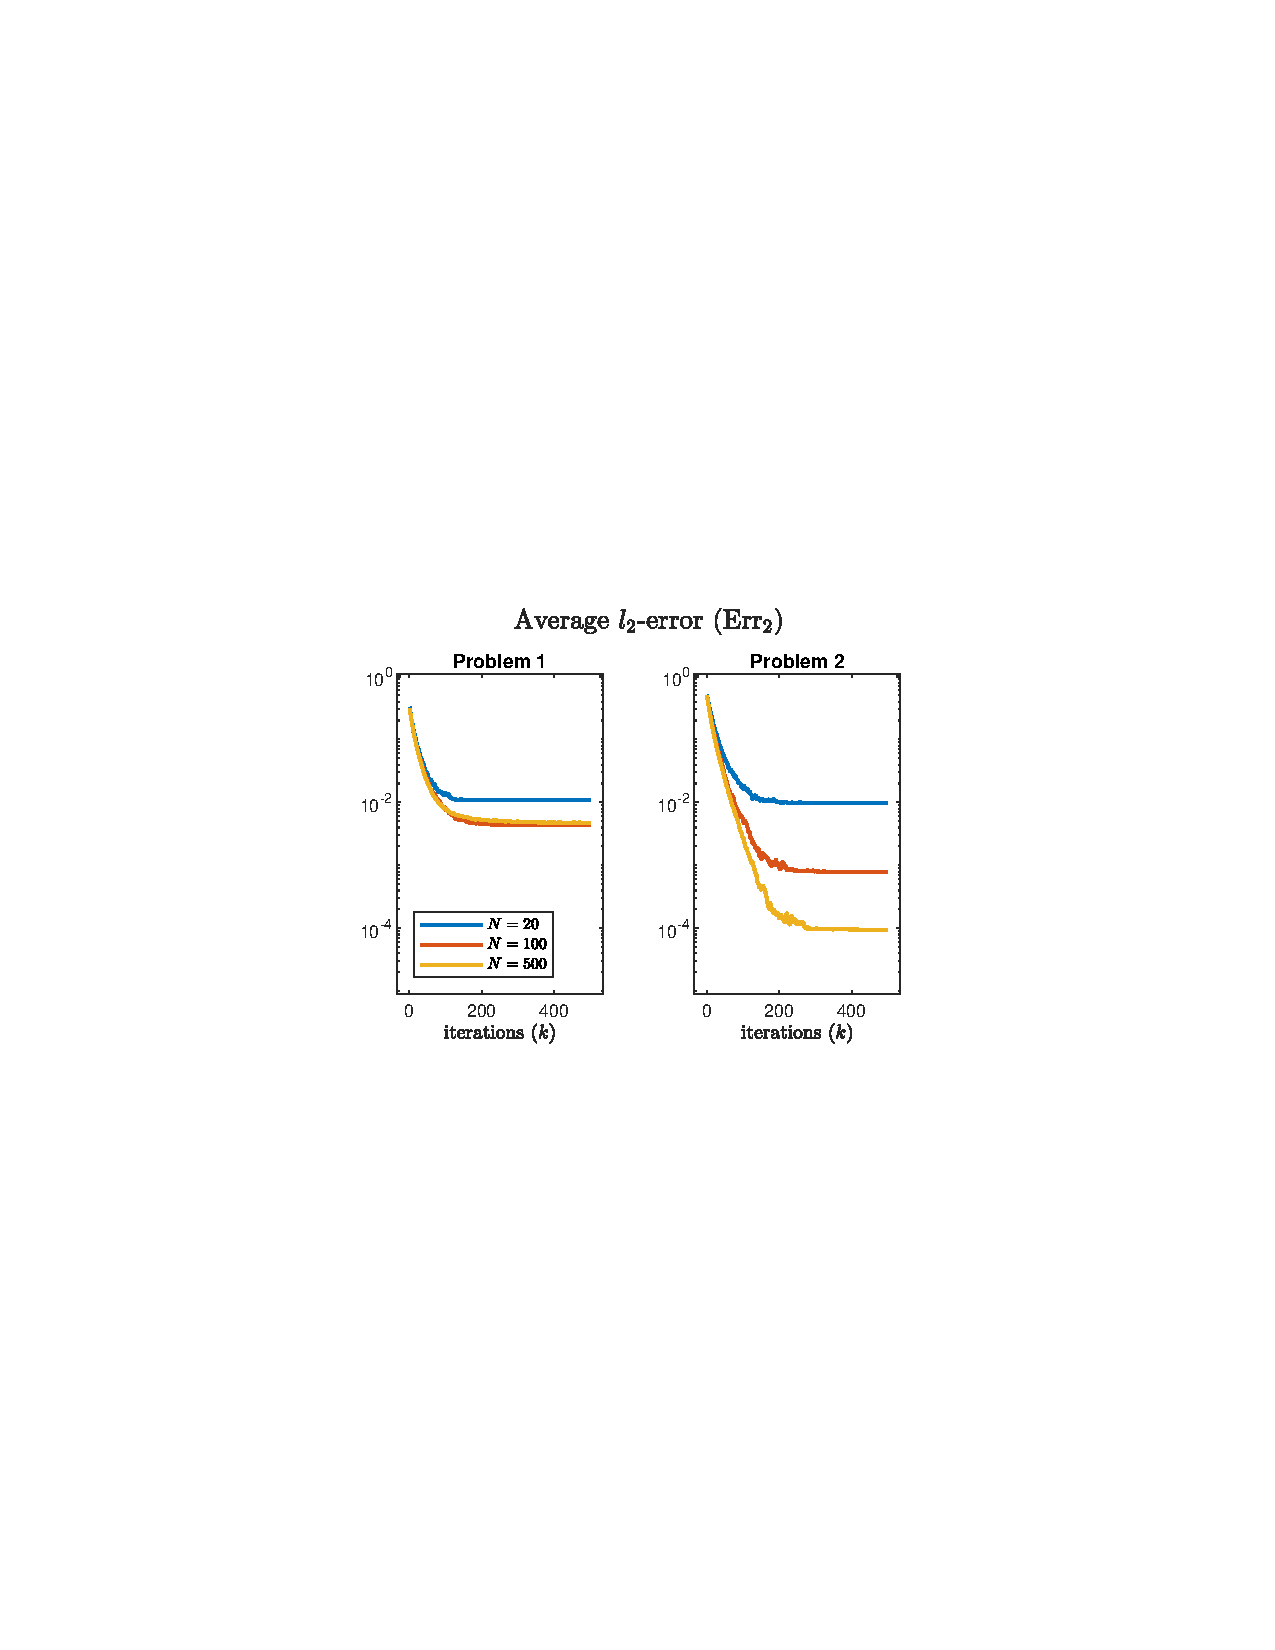
\includegraphics[trim=6cm 10cm 6cm 10.2cm, clip, width=3in]{ExperimentTile_aniso}%width=2.5in
\caption{Average $\ell_2$-error, as defined in \eqref{eq:err}, as function of the iterative step $k$ for Problem 1 and 2. Different population sizes $N$ are considered. Update rule given by \eqref{eq:iter}. Results averaged over 1000 runs.}
\label{fig:conv}
\end{figure}


In this section, we validate the suggested heuristic strategy on four bi-objective optimization test problems, that is with $m=2$. 
The first problem \cite{Pardalos2018} is given by 
\begin{align}
g(x_1,x_2) = \begin{pmatrix}
5(x_1 - 0.1)^2 + (x_2 - 0.1)^2
\\
(x_1 - 0.9)^2 + 5(x_2 - 0.9)^2
\end{pmatrix}
\end{align}
with $x \in [0,1]^2$, while the second one is the DEB2DK problem \cite{finding2004deb}, with one knee ($K=1$) and $d=2$. Problems 3 and 4 are taken form the test suit \cite[problems UF4, UF7]{zhang2008multiobjective} and can be scaled to different dimensions $d$. Given that Problems 2 and 3 are non-convex, we employ the Chebyschev norm approach by setting $p = \infty$ which, thanks to Theorem \ref{t:2}, is suitable for such problems. 

As in many multi-objective problems \cite{Pardalos2018}, the search space of each test consists of a different hypercube $D \subset \mathbb{R}^d$. Therefore, after every iteration we clip the vectors $X_k^i$ to ensure the agents will remain in the search space. Alternatively, a penalization term can be added to the objective function. The initial agents positions are uniformly sampled from $D$, $\rho_0 = \mathcal{U}(D)$, while the weights are deterministically chosen as $w^i = \left((i-1)\Delta w, 1 - (i-1)\Delta w \right)$ with $\Delta w = 1/(N-1)$.


%%OLD FIGURE BELOW

%\begin{figure*}[!t]
%\centering
%\subfloat{
\includegraphics[trim=7cm 10cm 7.3cm 10cm, clip, width=1.6in]{FIG/SingleSimulation_5aniso}
%%\label{fig_first_case}
%}
%\hfil
%\subfloat{
\includegraphics[trim=7cm 10cm 7.3cm 10cm, clip, width=1.6in]{FIG/SingleSimulation_10aniso}}
%\hfil
%\subfloat{\includegraphics[trim=7cm 10cm 7.3cm 10cm, clip, width=1.6in]{FIG/SingleSimulation_24_aniso_12}} %SingleSimulation_24aniso
%\hfil
%\subfloat{\includegraphics[trim=7cm 10cm 7.3cm 10cm, clip, width=1.6in]{FIG/SingleSimulation_27_aniso_6}} %SingleSimulation_27aniso
%\caption{Agents position at the end of a single run with $N=100, \sigma=4$ (Problem 1 and 2) and $N=300, \sigma =10$ (Problem 3 and 4). In red the solution $F_x$ and the Pareto front $F_g$ respectively. In Problems 3 and 4, $d=5$ and the greedy strategy \eqref{eq:greedy} is used.}
%\label{fig:pareto}
%\end{figure*}

\begin{figure*}[!t]
\centering
\subfloat[$d=2,\, N=100,\, \sigma = 4$]{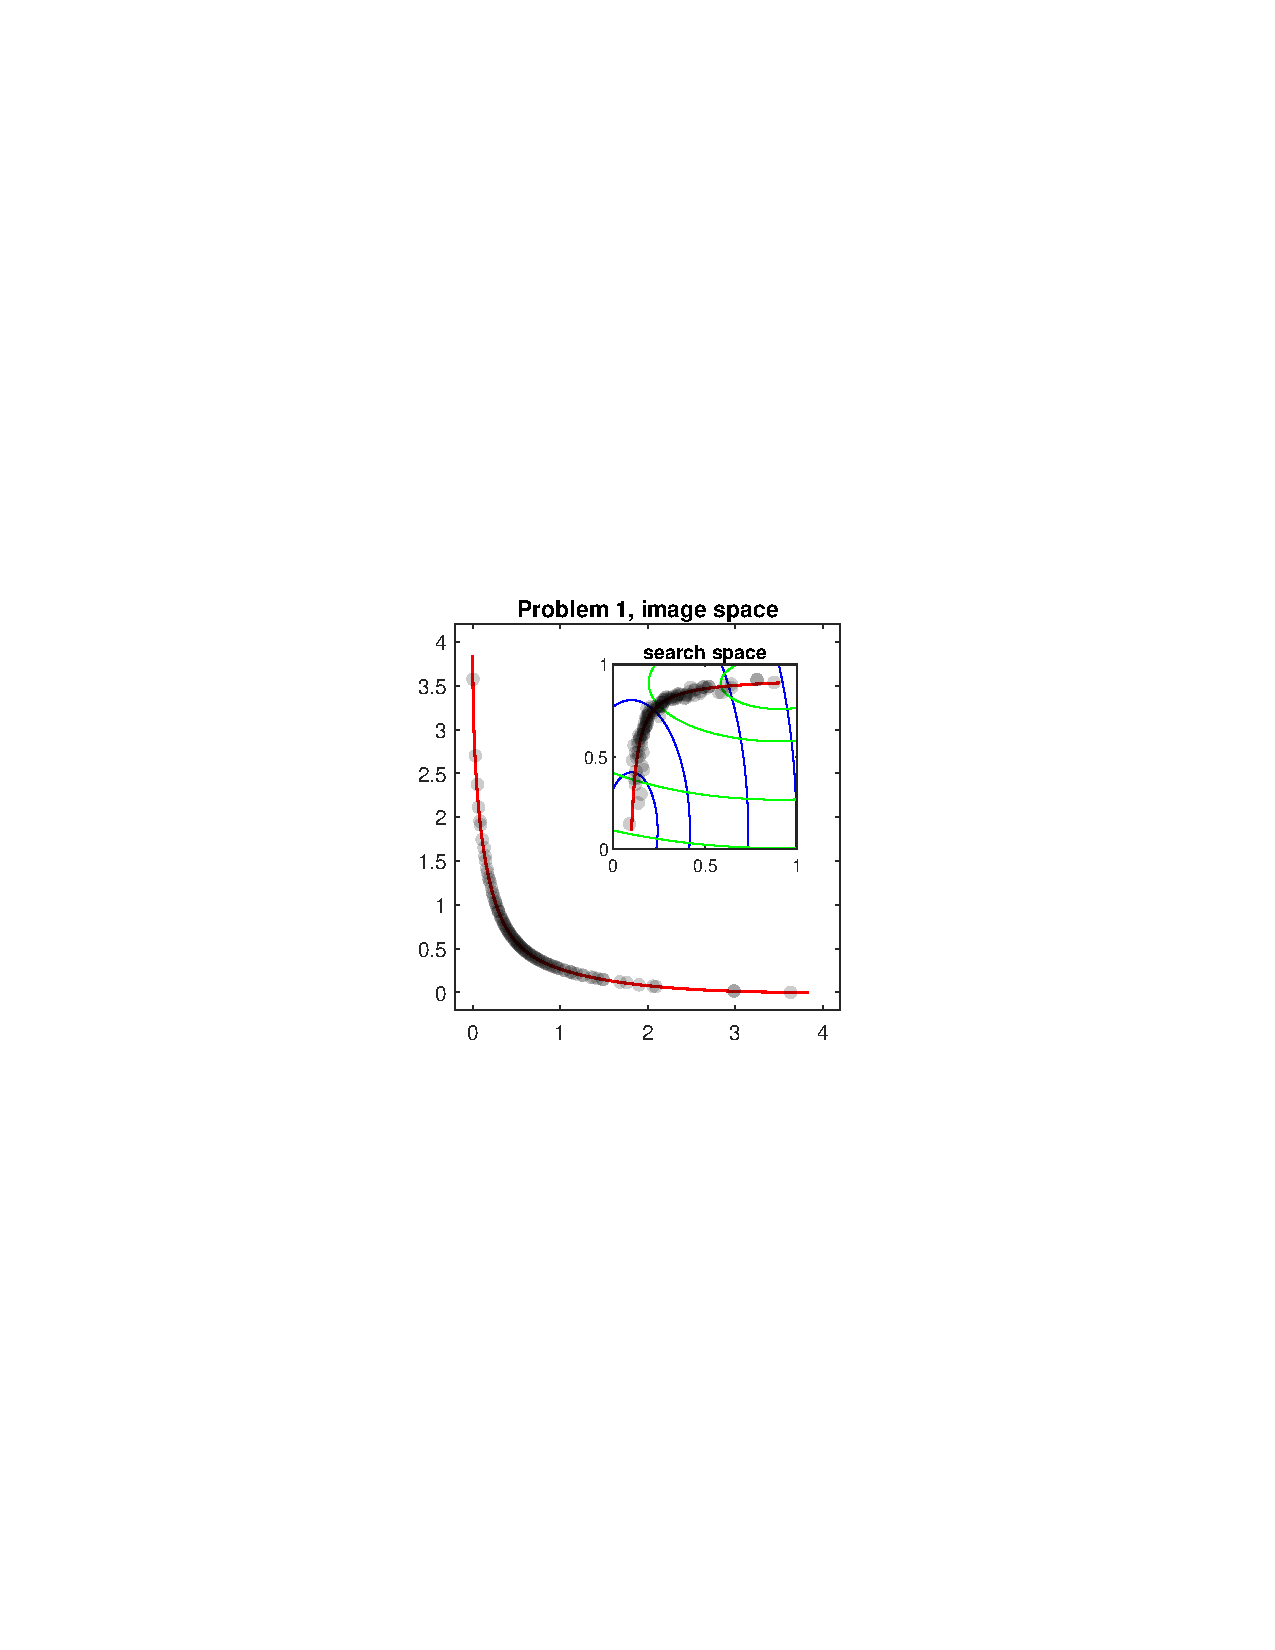
\includegraphics[trim=7cm 10cm 7.3cm 10cm, clip, width=1.6in]{SingleSimulation_5aniso}
\label{fig2a}
}
\hfil
\subfloat[$d=2,\, N=100,\, \sigma = 4$]{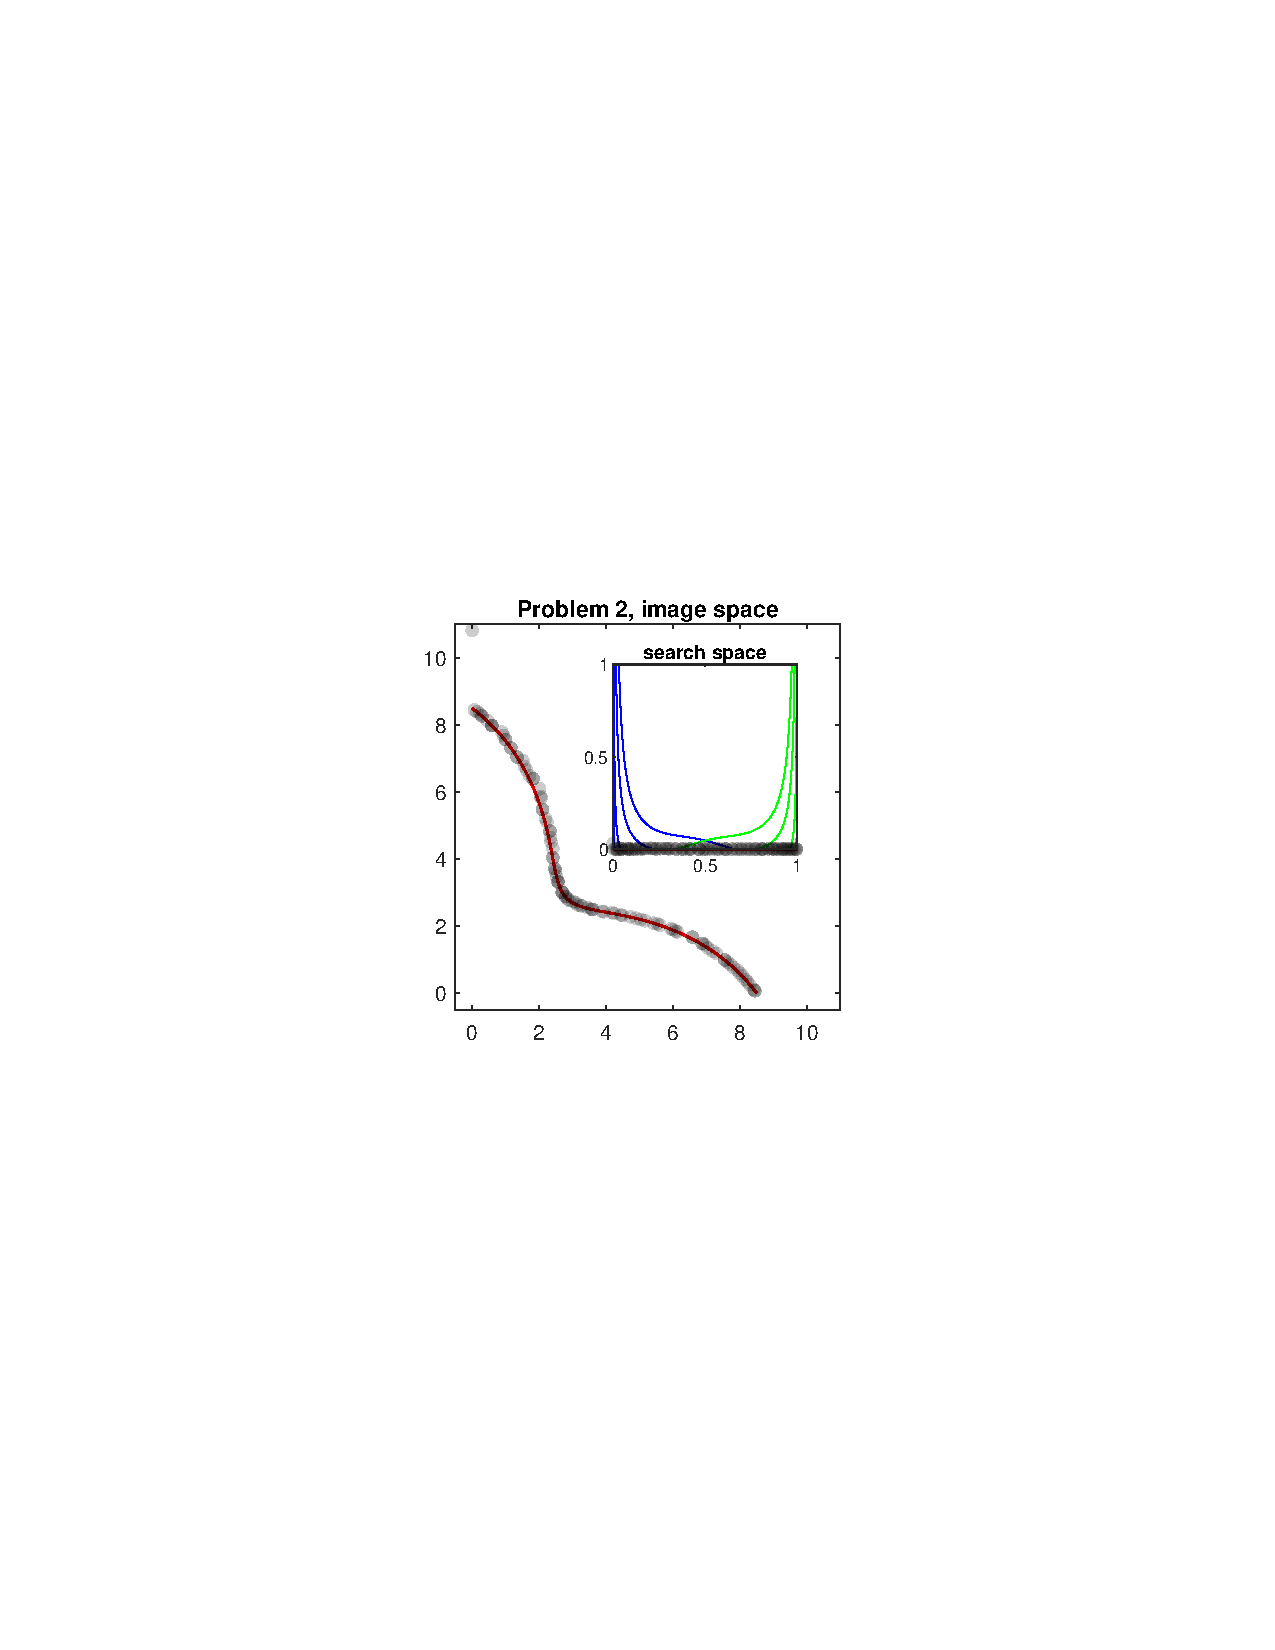
\includegraphics[trim=7cm 10cm 7.3cm 10cm, clip, width=1.6in]{SingleSimulation_10aniso} \label{fig2b}}
\hfil
\subfloat[$d=5,\, N=300,\, \sigma = 10$]{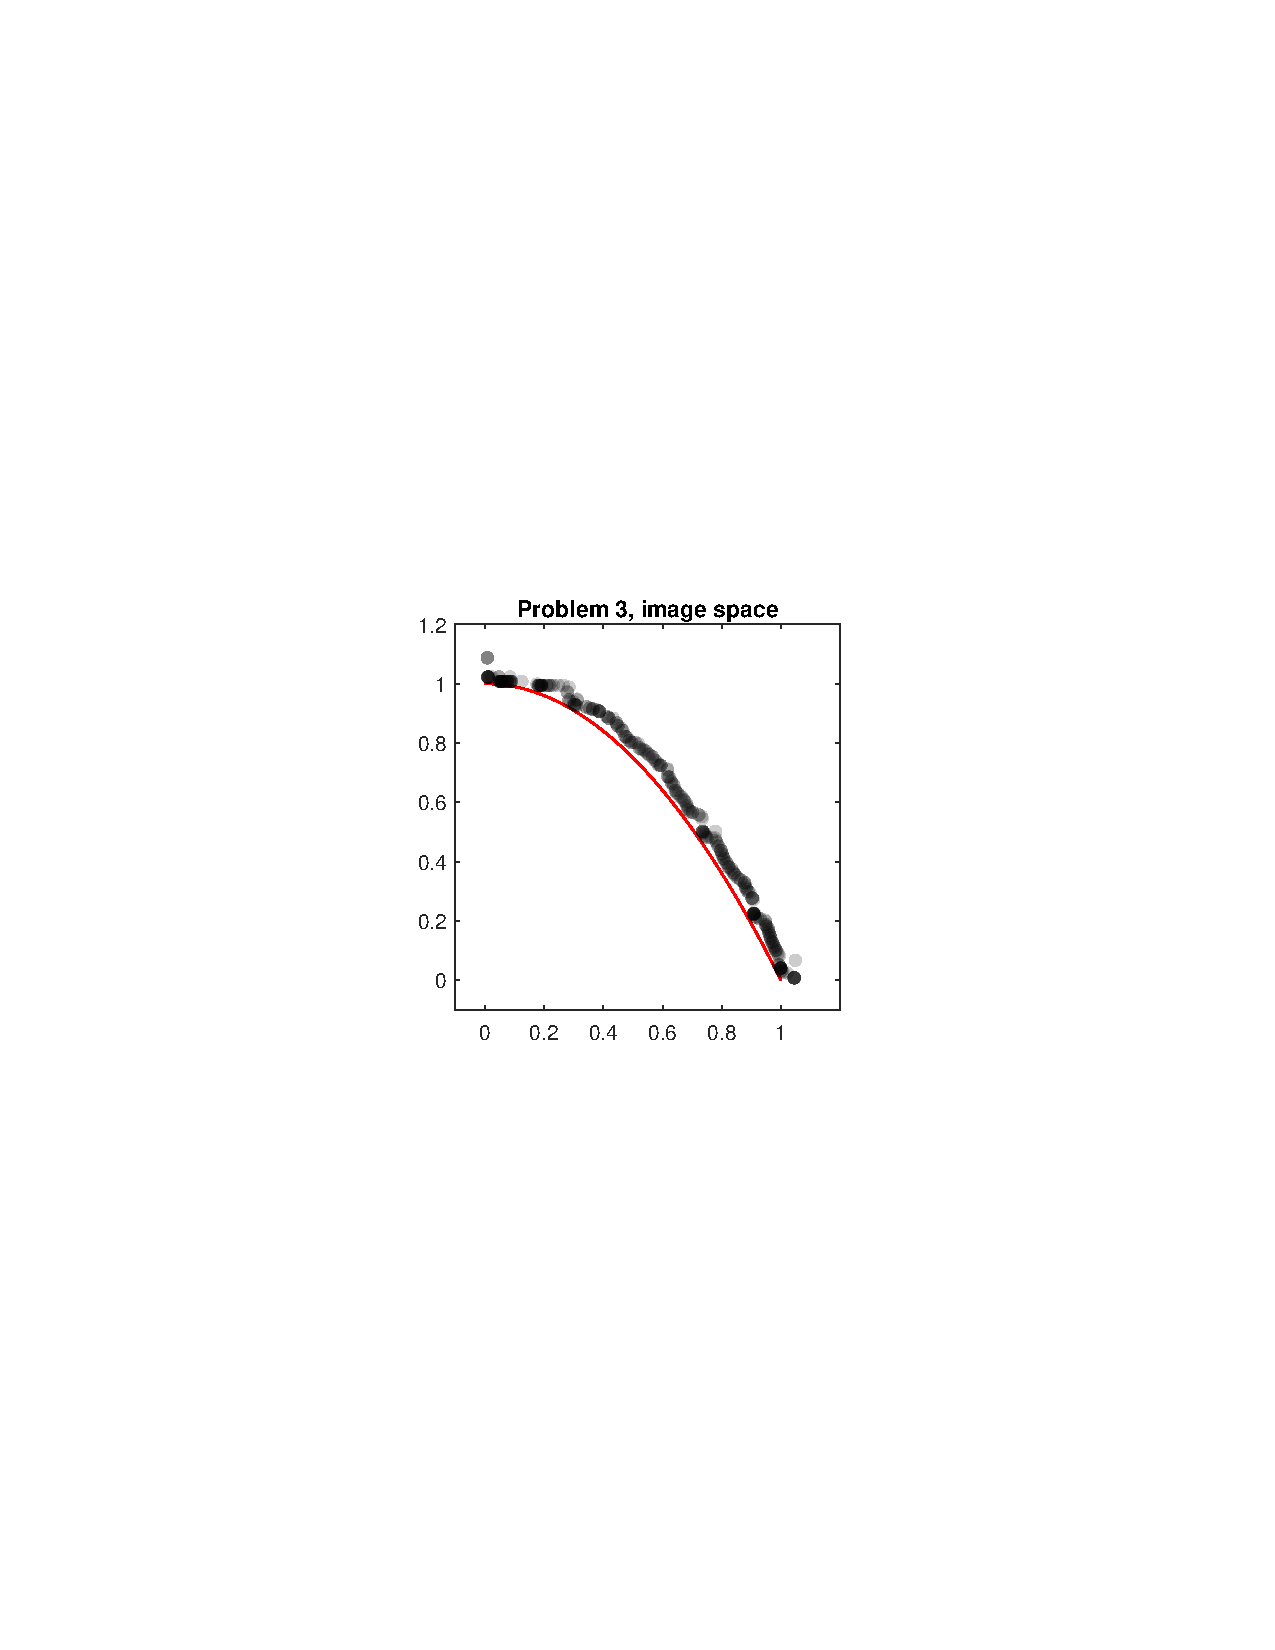
\includegraphics[trim=7cm 10cm 7.3cm 10cm, clip, width=1.6in]{SingleSimulation_24_aniso_10}\label{fig2c}} %SingleSimulation_24aniso
\hfil
\subfloat[$d=5,\, N=300,\, \sigma = 10$]{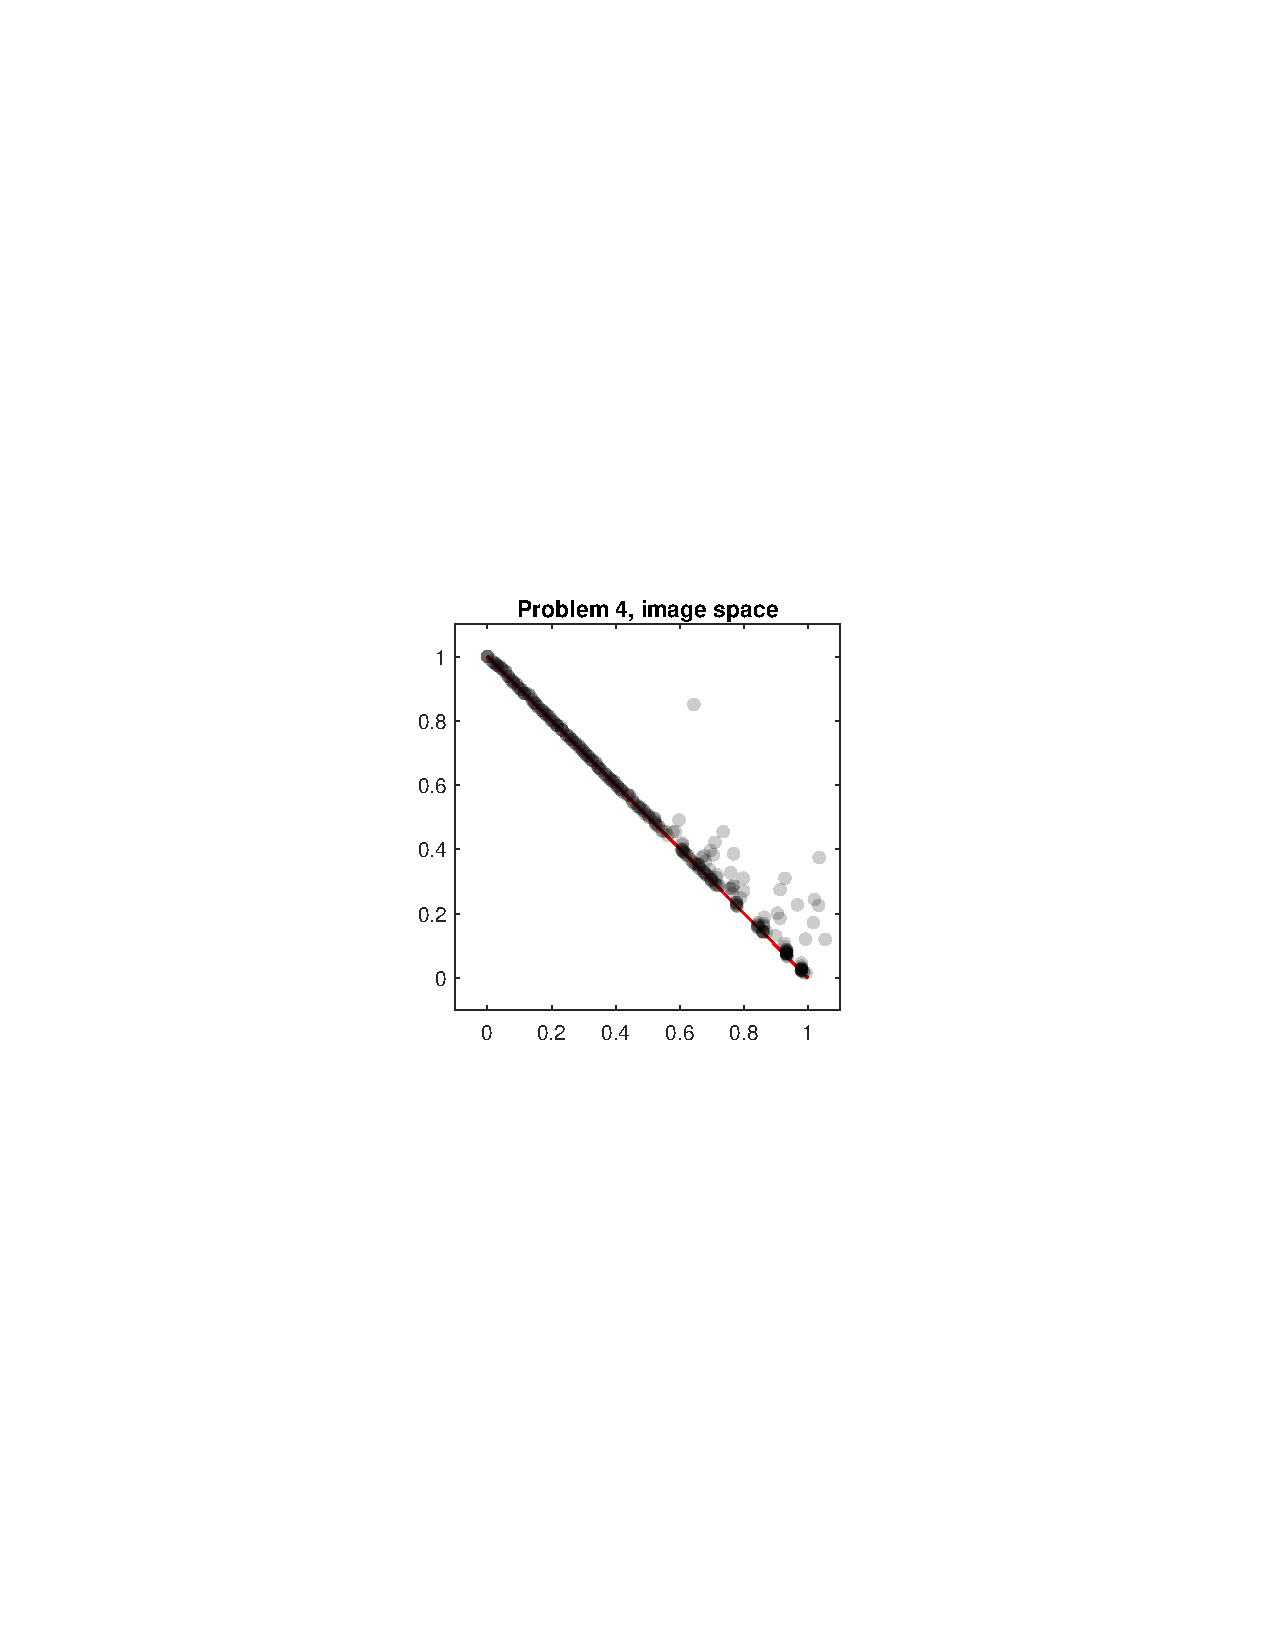
\includegraphics[trim=7cm 10cm 7.3cm 10cm, clip, width=1.6in]{SingleSimulation_27_aniso_10}\label{fig2d}} %SingleSimulation_27aniso
\caption{Agents position at the end of a single run, $k_{\max}=500$ . In red the Pareto front $F_g$ and, when $d=2$, the optimal points $F_x$. In Problems 3 and 4 the greedy strategy \eqref{eq:greedy} is used.}
\label{fig:pareto}
\end{figure*}



In similar multi-agent algorithms, the step size $\Delta t$ is typically of order between $0.1$ and $0.01$ \cite{pinnau2017consensus, carrillo2019consensus, benfenati2021binary}. In our experiments, we were able to reach higher accuracy with step size $\Delta t =0.01$.
Even though using adapting parameters is a common strategy to promote exploration at the beginning of the computation \cite{carrillo2019consensus,fhps20-2}, we test the algorithm mechanism by keeping $\lambda =1, \Delta t =0.01, \alpha = 10^{5}$ fixed. The exploration parameter is fixed to $\sigma=4$ for Problems 1 and 2, and $\sigma=10$ for higher dimensional problems. The agents evolve until a maximum number of iterations $k_{\textup{max}} $ is reached.

We first consider Problem 1 and 2, for which is possible to compute the solution of each sub-problem \eqref{pb:scal} with high accuracy.
Figs. \ref{fig:conv} show the average error $\textup{Err}_2$ for different population sizes $N$. We note that the agents converge quickly to the solution of the correspondent sub-problems, up to a certain accuracy. 

For the remaining part of the computation, the agent system is almost stationary. Indeed, once the $i$-th agent approximates the solution of the $i$-th problem better than the other agents, the convex combination $x_k^\alpha(w^i)$ is typically close to $X_k^i$ itself due to the Laplace principle. Note that, even though using small values of $\alpha$ would still evolve the dynamics, this would lead to a movement of positions towards the same point and an increase of the average error. This due the definition of $x_k^\alpha(w)$ as convex combination of the agents position. 

%Intuitively, in the limiting case of $\alpha=0$, it holds
%\[ x^\alpha_k (w) =  \bar X = \frac{1}N \sum_{i=1}^N X_k^i 
%\]
%for all $w \in \Omega$



As expected, employing larger number of agents allows to a better exploration of the search space and higher accuracy of the solution. Nevertheless, this improvement may be little, as shown in Fig. \ref{fig:conv} (left), where the accuracy reached with $N=100$ agents is almost as good as the one  reached with $N=500$. This can be explained by a known shortcoming of the scalarization strategy. Typically, taking uniformly distributed weights vectors does not guarantee equally distributed Pareto points, both in the search-space and in image-space \cite{Pardalos2018}. 


This is particularly evident for the Problem 1, see Fig. \ref{fig2a}, where the solutions are concentrated at the center (with respect to the symmetry axis). Indeed, the agents concentrate towards the center due to the combinatorial nature of $x^\alpha(w)$. This leads to a low accuracy 
solutions at the extrema of the Pareto front,
even for large population sizes. In Problem 2, this effect is less evident as the agents are better distributed over the front, see Fig. \ref{fig2b}. 

\begin{figure}[!b]
\centering
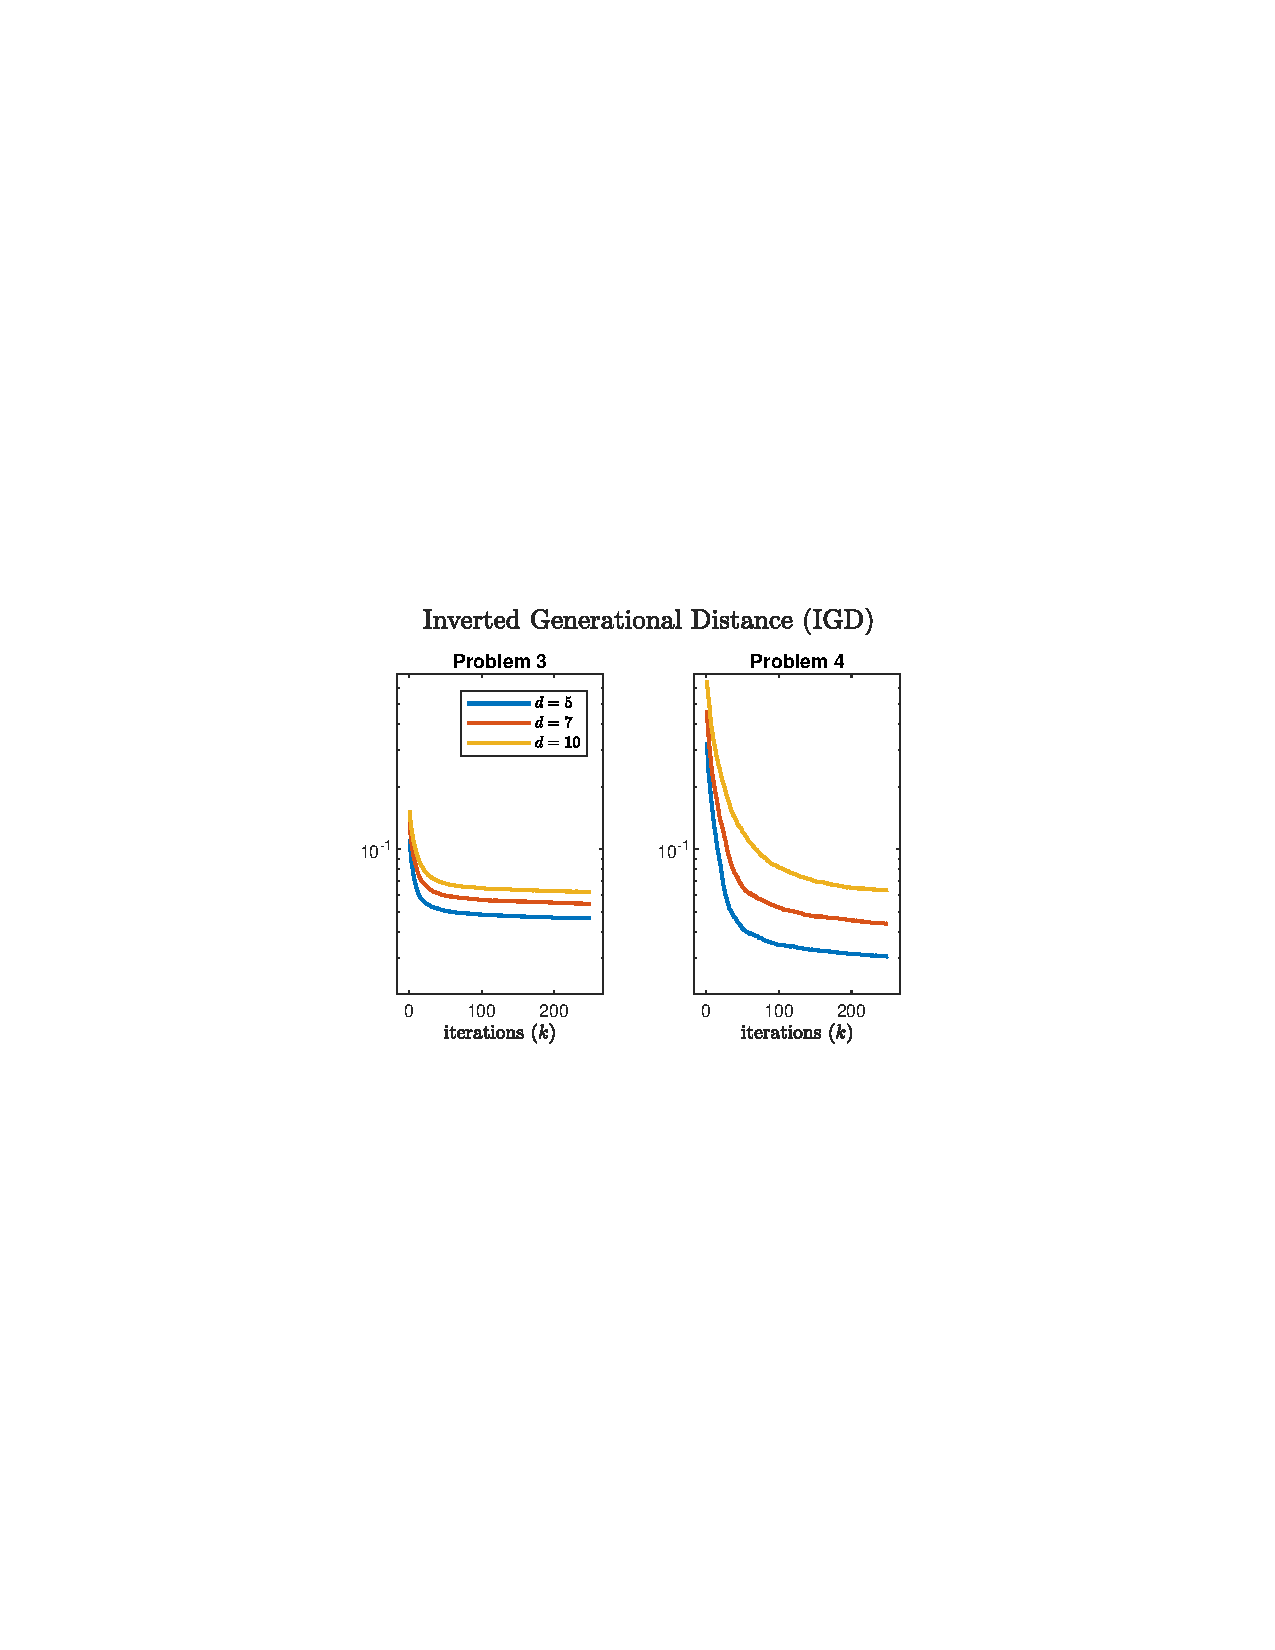
\includegraphics[trim=6cm 10cm 6cm 10.2cm, clip, width=3in]{CECexp_all_24_27}%width=2.5in
\caption{IGD metric as function of the iterative step $k$ for Problem 3 and 4. Different dimensions $d=5,7,10$ of the search space are considered, while $N=300$ is fixed.  Update rule given by \eqref{eq:greedy} (greedy strategy). Results averaged over 50 runs.}
%2.398648344710328e-04
\label{fig:dim}
\end{figure}



We test the proposed method with higher dimensional problems, where $d=5,7,10$. To improve the  algorithm performance, we employ a greedy strategy which updates the location of the $i$-th agent only if the new location improves the objective function value of the $i$-th sub-problem. This can be done by substituting the update rule \eqref{eq:iter} with
%\begin{equation}
\begin{align}
%X^i_{k+1} &= X^i_k + \lambda\Delta\, t H^i_k\, \left (x^\alpha_k(w^i) - X^i_k \right) \\
%& \hspace{2cm} + \sigma \Delta t\, H^i_k \,| x^\alpha_k(w^i) - X^i_k| B_k^i\, \\
%H^i_k & = H\left( G_p(X^i_k, w^i) - G_p(X^i_{k+1}, w^i) \right)
Y^i_{k+1} &= X^i_k + \lambda\Delta t\left (x^\alpha_k(w^i) - X^i_k \right) \notag
\\
&\hspace{1cm} + \sigma \sqrt{\Delta t} \sum_{l=1}^d (x^\alpha_k(w^i) - X^i_k)_l \, B_{k}^{i,l}\, \vec{e}_l 
\label{eq:greedy}
\\
X^i_{k+1} & =H\left( G_p(X^i_k, w^i) - G_p(Y^i_{k+1}, w^i)  \right) ( Y^i_{k+1} - X^i_k)  \notag \\
&\hspace{1cm} + X^i_k \notag
\end{align}
%\end{equation}
where $H$ is the Heaviside function ($H(x) = 0$ if $x\leq0$ and $1$ otherwise). We note that the above dynamics can also be described by a correspondent mean-field model, after an appropriate regularization of $H$. 
For simplicity, we omit it and refer to \cite{pinnau2017consensus, fornasier2021consensusbased} for more details. We remark the method might benefit from a mixed strategy where the greedy mechanism is gradually turned on, as in the Simulated Annealing algorithm \cite{kirkpatrick1983annealing}. We leave this investigation for future work.

Fig. \ref{fig:dim} shows the evolution of the Inverted Generational Distance (IGD) which is a common metric for multi-objective optimization tasks, as it measures both the convergence and the well-distribution of the points over the Pareto front \cite{cheng2012performance}. Even though the IGD metric is increasing together with the dimension, the method is able to converge towards the Pareto front with only $N=300$ agents in dimension $d=10$.


%
%\begin{figure*}
%\begin{subfigure}{0.5\columnwidth}
%\includegraphics[trim=6.8cm 10cm 7cm 10cm, clip, width=2.5in]{FIG/SingleSimulation_5_aniso}%width=2.5in
%\end{subfigure}
%\begin{subfigure}
%\includegraphics[trim=6.8cm 10cm 7cm 10cm, clip, width=2.5in]{FIG/SingleSimulation_10_aniso}
%\end{subfigure}
%\caption{Problem 1. Agents position at the end of a single run with $N=100$, and their images in the image-space. In red the solution $F_x$ and the Pareto front $F_g$ respectively.}
%\label{fig:sim5}
%\end{figure*}
%

%\begin{figure}[!t]
%\centering
%\includegraphics[trim=6.8cm 10cm 7cm 10cm, clip, width=2.5in]{FIG/SingleSimulation_10_aniso}%width=2.5in
%\caption{Problem 2. Agents position at the end of a single run with $N=100$, and their images in the image-space. In red the solution $F_x$ and the Pareto front $F_g$ respectively.}
%%2.398648344710328e-04
%\label{fig:sim10}
%\end{figure}





%\begin{figure}[!t]
%\centering
%\includegraphics[trim=7cm 10.5cm 7cm 10cm, clip, width=2.5in]{FIG/Experiment5}%width=2.5in
%\caption{Convergence behavior for different values of $N$ for the convex example. Results averaged over 50 runs.}
%\label{fig:conv5}
%\end{figure}
%
%
%\begin{figure}[!t]
%\centering
%\includegraphics[trim=7cm 10.5cm 7cm 10cm, clip, width=2.5in]{FIG/Experiment10}%width=2.5in
%\caption{Convergence behavior for different values of $N$ for the non-convex example. Results averaged over 50 runs.}
%\label{fig:conv10}
%\end{figure}




%\begin{figure}[thpb]
%      \centering
%      \framebox{\parbox{3in}{We suggest that you use a text box to insert a graphic (which is ideally a 300 dpi TIFF or EPS file, with all fonts embedded) because, in an document, this method is somewhat more stable than directly inserting a picture.}}
%      \framebox{\parbox{3in}}{ \includegraphics{FIG/SingleSimulation_5}} %[scale=1.0]
%      \caption{Inductance of oscillation winding on amorphous       magnetic core versus DC bias magnetic field}
%      \label{figurelabel}
%   \end{figure}
   
   
%\begin{itemize}
%\item Comment on how to choose the parameters and stopping criterion
%\item Definition of two examples (example 2 needs to be replaced with a mixed one)
%\item Comment on plots
%\item Remark on the difference between standard convergence metrics, like IGD, and $\textup{Err}_2(k)$.
%\end{itemize}

\section{CONCLUSIONS}
We proposed a multi-agent multi-objective algorithm which solves, at the same time, $N$ sub-problems generated by a scalarization strategy. We give a statistical description of the agents dynamics through the mean-field limit, which is given by the limit of the step-size $\Delta t \to 0$ and $N \to \infty$. Such approximation is an essential step to analytically study the algorithm's behavior.
Computational tests show the agents distribution over the Pareto front and the validity of the proposed approach.

The initial choice of uniform weights vectors is known to be non-optimal for a general multi-objective problem.  We observe that this may have a strong impact on the convergence. In future work, we plan of adding an interaction in the weights to mitigate this issue and obtain a better approximation of the Pareto front and, also, an higher accuracy in solution of the sub-problems.

%\balance
\IEEEtriggeratref{13}

%%%%%%%%%%%%%%%%%%%%%%%%%%
\begin{comment}
\section{INTRODUCTION}

This template provides authors with most of the formatting specifications needed for preparing electronic versions of their papers. All standard paper components have been specified for three reasons: (1) ease of use when formatting individual papers, (2) automatic compliance to electronic requirements that facilitate the concurrent or later production of electronic products, and (3) conformity of style throughout a conference proceedings. Margins, column widths, line spacing, and type styles are built-in; examples of the type styles are provided throughout this document and are identified in italic type, within parentheses, following the example. Some components, such as multi-leveled equations, graphics, and tables are not prescribed, although the various table text styles are provided. The formatter will need to create these components, incorporating the applicable criteria that follow.

\begin{theorem}
$x^2 = 0$
\end{theorem}

\section{PROCEDURE FOR PAPER SUBMISSION}

\subsection{Selecting a Template (Heading 2)}

First, confirm that you have the correct template for your paper size. This template has been tailored for output on the US-letter paper size. 
It may be used for A4 paper size if the paper size setting is suitably modified.

\subsection{Maintaining the Integrity of the Specifications}

The template is used to format your paper and style the text. All margins, column widths, line spaces, and text fonts are prescribed; please do not alter them. You may note peculiarities. For example, the head margin in this template measures proportionately more than is customary. This measurement and others are deliberate, using specifications that anticipate your paper as one part of the entire proceedings, and not as an independent document. Please do not revise any of the current designations

\section{MATH}

Before you begin to format your paper, first write and save the content as a separate text file. Keep your text and graphic files separate until after the text has been formatted and styled. Do not use hard tabs, and limit use of hard returns to only one return at the end of a paragraph. Do not add any kind of pagination anywhere in the paper. Do not number text heads-the template will do that for you.

Finally, complete content and organizational editing before formatting. Please take note of the following items when proofreading spelling and grammar:

\subsection{Abbreviations and Acronyms} Define abbreviations and acronyms the first time they are used in the text, even after they have been defined in the abstract. Abbreviations such as IEEE, SI, MKS, CGS, sc, dc, and rms do not have to be defined. Do not use abbreviations in the title or heads unless they are unavoidable.

\subsection{Units}

\begin{itemize}

\item Use either SI (MKS) or CGS as primary units. (SI units are encouraged.) English units may be used as secondary units (in parentheses). An exception would be the use of English units as identifiers in trade, such as 3.5-inch disk drive.
\item Avoid combining SI and CGS units, such as current in amperes and magnetic field in oersteds. This often leads to confusion because equations do not balance dimensionally. If you must use mixed units, clearly state the units for each quantity that you use in an equation.
\item Do not mix complete spellings and abbreviations of units:  Wb/m2  or  webers per square meter , not  webers/m2 .  Spell out units when they appear in text: . . . a few henries , not . . . a few H .
\item Use a zero before decimal points:  0.25 , not .25 . Use  cm3 , not  cc . (bullet list)

\end{itemize}


\subsection{Equations}

The equations are an exception to the prescribed specifications of this template. You will need to determine whether or not your equation should be typed using either the Times New Roman or the Symbol font (please no other font). To create multileveled equations, it may be necessary to treat the equation as a graphic and insert it into the text after your paper is styled. Number equations consecutively. Equation numbers, within parentheses, are to position flush right, as in (1), using a right tab stop. To make your equations more compact, you may use the solidus ( / ), the exp function, or appropriate exponents. Italicize Roman symbols for quantities and variables, but not Greek symbols. Use a long dash rather than a hyphen for a minus sign. Punctuate equations with commas or periods when they are part of a sentence, as in

$$
\alpha + \beta = \chi \eqno{(1)}
$$

Note that the equation is centered using a center tab stop. Be sure that the symbols in your equation have been defined before or immediately following the equation. Use (1), not  Eq. (1) or  equation (1), except at the beginning of a sentence:  Equation (1) is . . .

\subsection{Some Common Mistakes}
\begin{itemize}


\item The word  data  is plural, not singular.
\item The subscript for the permeability of vacuum ?0, and other common scientific constants, is zero with subscript formatting, not a lowercase letter  o .
\item In American English, commas, semi-/colons, periods, question and exclamation marks are located within quotation marks only when a complete thought or name is cited, such as a title or full quotation. When quotation marks are used, instead of a bold or italic typeface, to highlight a word or phrase, punctuation should appear outside of the quotation marks. A parenthetical phrase or statement at the end of a sentence is punctuated outside of the closing parenthesis (like this). (A parenthetical sentence is punctuated within the parentheses.)
\item A graph within a graph is an  inset , not an  insert . The word alternatively is preferred to the word  alternately  (unless you really mean something that alternates).
\item Do not use the word  essentially  to mean  approximately  or  effectively .
\item In your paper title, if the words  that uses  can accurately replace the word  using , capitalize the  u ; if not, keep using lower-cased.
\item Be aware of the different meanings of the homophones  affect  and  effect ,  complement  and  compliment ,  discreet  and  discrete ,  principal  and  principle .
\item Do not confuse  imply  and  infer .
\item The prefix  non  is not a word; it should be joined to the word it modifies, usually without a hyphen.
\item There is no period after the  et  in the Latin abbreviation  et al..
\item The abbreviation  i.e. means  that is , and the abbreviation  e.g. means  for example .

\end{itemize}


\section{USING THE TEMPLATE}

Use this sample document as your LaTeX source file to create your document. Save this file as {\bf root.tex}. You have to make sure to use the cls file that came with this distribution. If you use a different style file, you cannot expect to get required margins. Note also that when you are creating your out PDF file, the source file is only part of the equation. {\it Your \TeX\ $\rightarrow$ PDF filter determines the output file size. Even if you make all the specifications to output a letter file in the source - if your filter is set to produce A4, you will only get A4 output. }

It is impossible to account for all possible situation, one would encounter using \TeX. If you are using multiple \TeX\ files you must make sure that the ``MAIN`` source file is called root.tex - this is particularly important if your conference is using PaperPlaza's built in \TeX\ to PDF conversion tool.

\subsection{Headings, etc}

Text heads organize the topics on a relational, hierarchical basis. For example, the paper title is the primary text head because all subsequent material relates and elaborates on this one topic. If there are two or more sub-topics, the next level head (uppercase Roman numerals) should be used and, conversely, if there are not at least two sub-topics, then no subheads should be introduced. Styles named  Heading 1 ,  Heading 2 ,  Heading 3 , and  Heading 4  are prescribed.

\subsection{Figures and Tables}

Positioning Figures and Tables: Place figures and tables at the top and bottom of columns. Avoid placing them in the middle of columns. Large figures and tables may span across both columns. Figure captions should be below the figures; table heads should appear above the tables. Insert figures and tables after they are cited in the text. Use the abbreviation  Fig. 1 , even at the beginning of a sentence.

\begin{table}[h]
\caption{An Example of a Table}
\label{table_example}
\begin{center}
\begin{tabular}{|c||c|}
\hline
One & Two\\
\hline
Three & Four\\
\hline
\end{tabular}
\end{center}
\end{table}


   \begin{figure}[thpb]
      \centering
      %\framebox{\parbox{3in}{We suggest that you use a text box to insert a graphic (which is ideally a 300 dpi TIFF or EPS file, with all fonts embedded) because, in an document, this method is somewhat more stable than directly inserting a picture.}}
      \includegraphics[scale=1.0]{figurefile}
      \caption{Inductance of oscillation winding on amorphous
       magnetic core versus DC bias magnetic field}
      \label{figurelabel}
   \end{figure}
   

Figure Labels: Use 8 point Times New Roman for Figure labels. Use words rather than symbols or abbreviations when writing Figure axis labels to avoid confusing the reader. As an example, write the quantity  Magnetization , or  Magnetization, M , not just  M . If including units in the label, present them within parentheses. Do not label axes only with units. In the example, write  Magnetization (A/m) or  Magnetization {A[m(1)]}, not just  A/m . Do not label axes with a ratio of quantities and units. For example, write  Temperature (K), not  Temperature/K.

\section{CONCLUSIONS}

A conclusion section is not required. Although a conclusion may review the main points of the paper, do not replicate the abstract as the conclusion. A conclusion might elaborate on the importance of the work or suggest applications and extensions. 

\addtolength{\textheight}{-12cm}   % This command serves to balance the column lengths
                                  % on the last page of the document manually. It shortens
                                  % the textheight of the last page by a suitable amount.
                                  % This command does not take effect until the next page
                                  % so it should come on the page before the last. Make
                                  % sure that you do not shorten the textheight too much.

%%%%%%%%%%%%%%%%%%%%%%%%%%%%%%%%%%%%%%%%%%%%%%%%%%%%%%%%%%%%%%%%%%%%%%%%%%%%%%%%



%%%%%%%%%%%%%%%%%%%%%%%%%%%%%%%%%%%%%%%%%%%%%%%%%%%%%%%%%%%%%%%%%%%%%%%%%%%%%%%%



%%%%%%%%%%%%%%%%%%%%%%%%%%%%%%%%%%%%%%%%%%%%%%%%%%%%%%%%%%%%%%%%%%%%%%%%%%%%%%%%
\section*{APPENDIX}

Appendixes should appear before the acknowledgment.

\section*{ACKNOWLEDGMENT}

The preferred spelling of the word  acknowledgment  in America is without an  e  after the  g . Avoid the stilted expression,  One of us (R. B. G.) thanks . . .  Instead, try  R. B. G. thanks . Put sponsor acknowledgments in the unnumbered footnote on the first page.



%%%%%%%%%%%%%%%%%%%%%%%%%%%%%%%%%%%%%%%%%%%%%%%%%%%%%%%%%%%%%%%%%%%%%%%%%%%%%%%%

References are important to the reader; therefore, each citation must be complete and correct. If at all possible, references should be commonly available publications.
\end{comment}


\bibliographystyle{IEEEtran}
\bibliography{IEEEabrv,IEEEexample}



%\begin{thebibliography}{99}
%
%\bibitem{c1} G. O. Young,  Synthetic structure of industrial plastics (Book style with paper title and editor), 	in Plastics, 2nd ed. vol. 3, J. Peters, Ed.  New York: McGraw-Hill, 1964, pp. 15 64.
%\bibitem{c2} W.-K. Chen, Linear Networks and Systems (Book style).	Belmont, CA: Wadsworth, 1993, pp. 123 135.
%\bibitem{c3} H. Poor, An Introduction to Signal Detection and Estimation.   New York: Springer-Verlag, 1985, ch. 4.
%\bibitem{c4} B. Smith,  An approach to graphs of linear forms (Unpublished work style), unpublished.
%\bibitem{c5} E. H. Miller,  A note on reflector arrays (Periodical style Accepted for publication), IEEE Trans. Antennas Propagat., to be publised.
%\bibitem{c6} J. Wang,  Fundamentals of erbium-doped fiber amplifiers arrays (Periodical style Submitted for publication), IEEE J. Quantum Electron., submitted for publication.
%\bibitem{c7} C. J. Kaufman, Rocky Mountain Research Lab., Boulder, CO, private communication, May 1995.
%\bibitem{c8} Y. Yorozu, M. Hirano, K. Oka, and Y. Tagawa,  Electron spectroscopy studies on magneto-optical media and plastic substrate interfaces(Translation Journals style), IEEE Transl. J. Magn.Jpn., vol. 2, Aug. 1987, pp. 740 741 [Dig. 9th Annu. Conf. Magnetics Japan, 1982, p. 301].
%\bibitem{c9} M. Young, The Techincal Writers Handbook.  Mill Valley, CA: University Science, 1989.
%\bibitem{c10} J. U. Duncombe,  Infrared navigation Part I: An assessment of feasibility (Periodical style), IEEE Trans. Electron Devices, vol. ED-11, pp. 34 39, Jan. 1959.
%\bibitem{c11} S. Chen, B. Mulgrew, and P. M. Grant,  A clustering technique for digital communications channel equalization using radial basis function networks, IEEE Trans. Neural Networks, vol. 4, pp. 570 578, July 1993.
%\bibitem{c12} R. W. Lucky,  Automatic equalization for digital communication, Bell Syst. Tech. J., vol. 44, no. 4, pp. 547 588, Apr. 1965.
%\bibitem{c13} S. P. Bingulac,  On the compatibility of adaptive controllers (Published Conference Proceedings style), in Proc. 4th Annu. Allerton Conf. Circuits and Systems Theory, New York, 1994, pp. 8 16.
%\bibitem{c14} G. R. Faulhaber,  Design of service systems with priority reservation, in Conf. Rec. 1995 IEEE Int. Conf. Communications, pp. 3 8.
%\bibitem{c15} W. D. Doyle,  Magnetization reversal in films with biaxial anisotropy, in 1987 Proc. INTERMAG Conf., pp. 2.2-1 2.2-6.
%\bibitem{c16} G. W. Juette and L. E. Zeffanella,  Radio noise currents n short sections on bundle conductors (Presented Conference Paper style), presented at the IEEE Summer power Meeting, Dallas, TX, June 22 27, 1990, Paper 90 SM 690-0 PWRS.
%\bibitem{c17} J. G. Kreifeldt,  An analysis of surface-detected EMG as an amplitude-modulated noise, presented at the 1989 Int. Conf. Medicine and Biological Engineering, Chicago, IL.
%\bibitem{c18} J. Williams,  Narrow-band analyzer (Thesis or Dissertation style), Ph.D. dissertation, Dept. Elect. Eng., Harvard Univ., Cambridge, MA, 1993. 
%\bibitem{c19} N. Kawasaki,  Parametric study of thermal and chemical nonequilibrium nozzle flow, M.S. thesis, Dept. Electron. Eng., Osaka Univ., Osaka, Japan, 1993.
%\bibitem{c20} J. P. Wilkinson,  Nonlinear resonant circuit devices (Patent style), U.S. Patent 3 624 12, July 16, 1990. 
%
%
%
%\end{thebibliography}
%



\end{document}
